%
% This is one of the samples from the lawtex package:
% http://lawtex.sourceforge.net/
% LawTeX is licensed under the GNU General Public License 
%
\pdfminorversion=7
\providecommand{\documentclassflag}{}
\documentclass[12pt,\documentclassflag]{michiganCourtOfAppealsBrief} 
\usepackage{etoolbox}
\usepackage[margin=1in]{geometry}
\usepackage{newcent,microtype}
\usepackage{setspace,xcolor}
\usepackage{trace}
\usepackage[T1]{fontenc}
\usepackage{pdfpages}
%\usepackage[hyperindex=false,linkbordercolor=white]{hyperref}
\makeandletter% use \makeandtab to turn off

% Use this to show a line grid-
% \usepackage[fontsize=12pt,baseline=24pt,lines=27]{grid}
% \usepackage{atbegshi,picture,xcolor} % https://tex.stackexchange.com/a/191004/135718
% \AtBeginShipout{%
%   \AtBeginShipoutUpperLeft{%
%     {\color{red}%
%     \put(\dimexpr -1in-\oddsidemargin,%
%          -\dimexpr 1in+\topmargin+\headheight+\headsep+\topskip)%
%       {%
%        \vtop to\dimexpr\vsize+\baselineskip{%
%          \hrule%
%          \leaders\vbox to\baselineskip{\hrule width\hsize\vfill}\vfill%
%        }%
%       }%
%   }}%
% }
%   \linespread{1}

\usepackage[modulo]{lineno}% use \linenumbers to show line numbers, see https://texblog.org/2012/02/08/adding-line-numbers-to-documents/

\chardef\_=`_% https://tex.stackexchange.com/a/301984/135718 

\begin{document}
\singlespacing
 
\def\mathieuGast{\cite[s]{MCL 211.27(2)}}%

\newmisc{STC Bulletin 7 of 2014}{Michigan State Tax Commission (STC) Bulletin No. 7 of 2014 (Mathieu Gast Act)}

\newcommand{\makeAbbreviation}[3]{% ensure that the frsit time an abbreviated word is used, it is presented in long form, and after that in short form. 1: command name, 2: short name, 3: long name
  \IfBeginWith{#3}{#2}{%
    \newcommand{#1}[0]{#3\renewcommand{#1}[0]{#2}}}{%
    \newcommand{#1}[0]{#3 (#2)\renewcommand{#1}[0]{#2}}}}

\makeAbbreviation{\MLS}{MLS}{Multiple Listing Service}
\makeAbbreviation{\MTT}{MTT}{Michigan Tax Tribunal}
\makeAbbreviation{\STC}{STC}{State Tax Commission}
%\makeAbbreviation{\FOJ}{FOJ}{First Final Opinion and Judgment (2017)}
\makeAbbreviation{\FOJ}{FOJ}{Second Final Opinion and Judgment (2018)}
\makeAbbreviation{\POJ}{POJ}{Proposed Opinion and Judgment}
\makeAbbreviation{\orderDenying}{Order Denying Reconsideration}{Order Denying Petitioner's Motion for Reconsideration}
\makeAbbreviation{\repairs}{List of Repairs}{List of Repairs, filed by Appellant with the Tax Tribunal on 9/6/2018}
\makeAbbreviation{\mlsprintout}{MLS Printout}{MLS Printout, filed by Appellant/Petitioner with Tax Tribunal on 9/7/2016}
\makeAbbreviation{\explanatoryLetter}{Explanatory Letter}{Explanatory Letter submitted by Appellant to the Tax Tribunal on 9/6/2018}

\begin{centering}
\bf\scshape State of Michigan\\In the Court of Appeals\\Detroit Office\\~\\ 
\rm 

\makeandtab
\begin{tabular}{p{.45\textwidth}|p{.45\textwidth}}
\cline{1-1}
  {~

  \raggedright Daniel Patru,\par
  \hfill\textit{Appellant,}
  \vspace{.5\baselineskip}
  \centerline{v}
  \vspace{.5\baselineskip}
  \raggedright City of Wayne,\par
  \hfill\textit{Appellee.}
  
  ~} &  {
      \hfill Court of Appeals No. 346894\par
      \hfill Lower Court No. 16-001828-TT\par\vspace{\baselineskip}
      \hfill \textbf{Appellant's Brief}\par
      \hfill \textbf{Proof of Service}
  }
  \\ \cline{1-1}\vspace{2mm}
  Daniel Patru, P74387, Appellant\newline%
  3309 Solway\newline%
  Knoxville, TN 37931\newline%
  (734) 274-9624\newline\newline%
  City of Wayne, Appellee\newline%
  3355 South Wayne Rd,\newline%
  Wayne, MI 48184\newline%
  (734) 722-2000%
  % \end{verbatim}
  & \\ 
\end{tabular}
\makeandletter

\end{centering}

\pagestyle{romanparen}
\pagenumbering{roman}
\newpage 

\section*{Table of Contents}

\tableofcontents

%\newpage
\pagestyle{plain}
\pagenumbering{arabic}

\parindent=2.5em
\doublespacing
% \linenumbers
\section{cover sheet}%

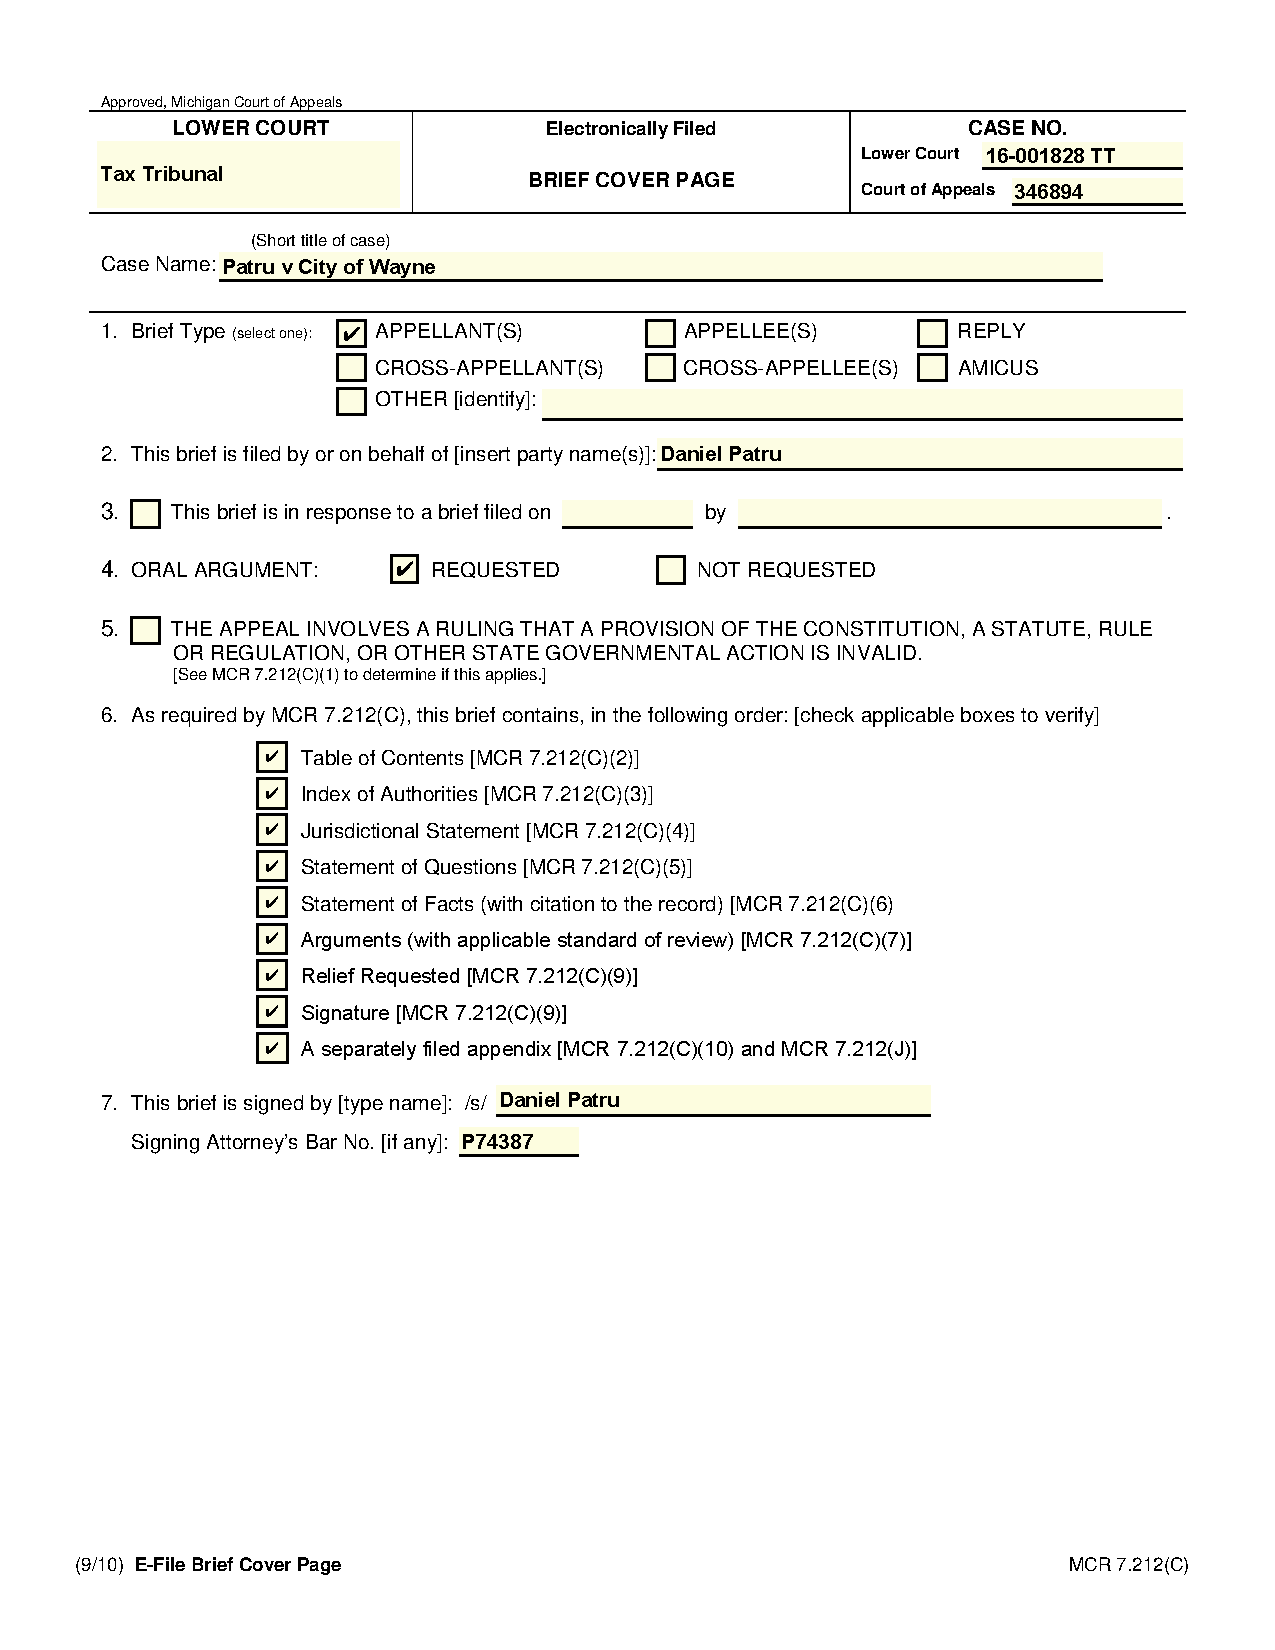
\includepdf[addtotoc={1,section,1,FirstSectionEntry,p1}]{COAE-FileBriefCoverSheet.pdf}
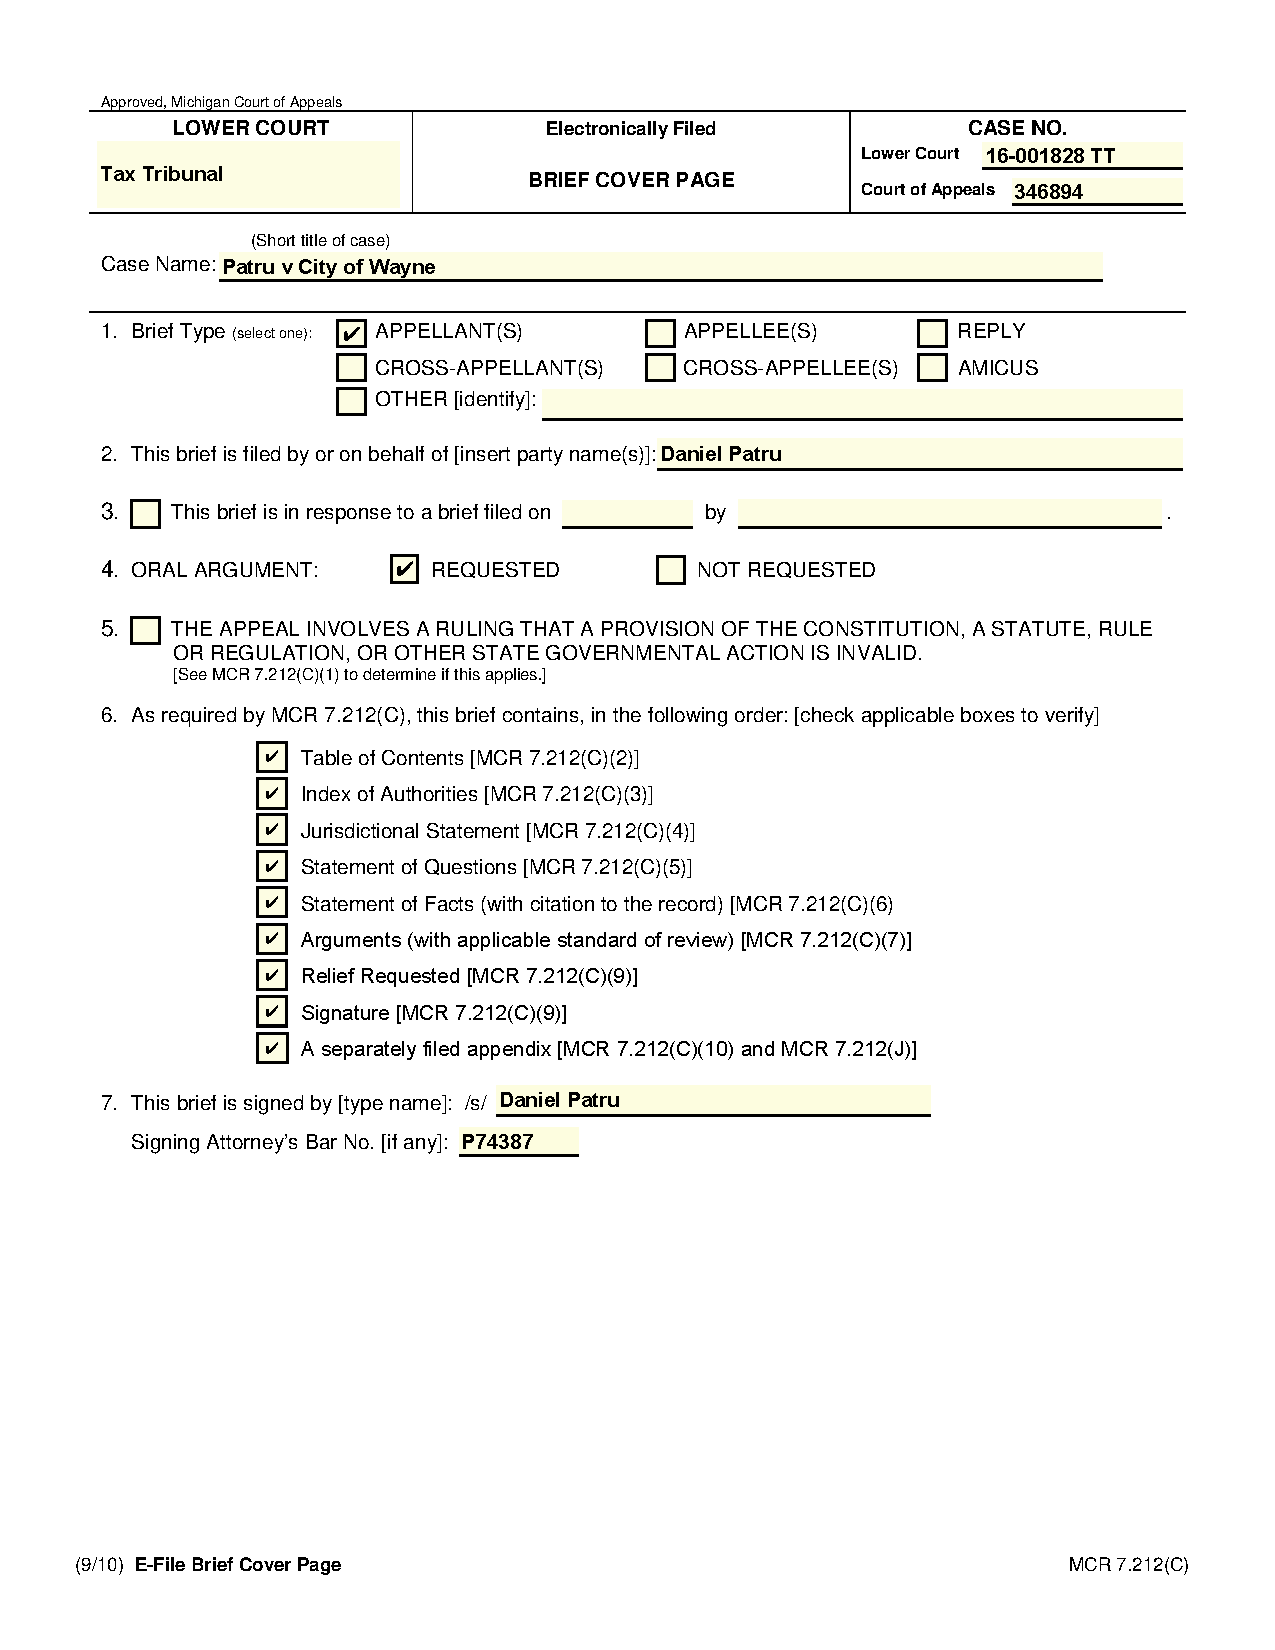
\includepdf[]{COAE-FileBriefCoverSheet.pdf}


\vspace{1\baselineskip}

{ \setlength{\leftskip}{3.5in}

  Respectfully Submitted,

  /s/ Daniel Patru

  2/15/2019

  \setlength{\leftskip}{0pt}}

\newpage\empty% we need a new page so that the index entries on the last
        % page get written out to the right file.
\end{document}


%%% Local Variables:
%%% mode: latex
%%% TeX-master: t
%%% End:
